\chapter{ Theoretical background }
At the end of the last chapter we announced the problem we want to study, the ultra-orthogonality property. Particularly we showed how this property is connected to the problem of equilibration as an instantaneous process rather. We also saw that ultra-orthogonality emerged as a direct consequence of typicality, hence, it is a general property of quantum systems. The purpose of this chapter is to provide the necessary theoretical background to study ultra-orthogonality for the specific case of fermionic systems.\\
\indent In this chapter we introduce the concepts of quasi-free fermionic models on a lattice and present Majorana fermions to define the fermionic covariance matrix and how this formalism can be used to develop some standard calculations on the diagonalising of the Hamiltonian of the one-dimensional $XY$ model, and we will discuss how is possible to treat excited states in as well local reduced states in this model. Since part of this work is dedicated to show an explicit connection between a special case of fermionic systems and code theory, the second part of this chapter will be dedicated to introduce some concepts of code theory that will allows us to make the explicit connection between code theory and fermionic system in the third chapter.

\section{Fermionic quadratic Hamiltonian}
In many areas of physics one has to deal with solving quantum many body problems. This is often a computationally difficult if not an impossible task. However, the cases that can be analytically solved are well-known, and have been a subject of study\cite{noauthor_density_2007,niu_majorana_2012,reyes-lega_aspects_2016,chung_density-matrix_2001,leijnse_introduction_2012, molinari_notes_2017,botero_bcs-like_2004, bravyi_lagrangian_2004, lieb_two_1961, latorre_ground_2004, katsura_statistical_1962, barouch_statistical_1971, barouch_statistical_1970}. It has been found that a wide class of complicated Hamiltonians with many-body interactions can often be mapped onto Hamiltonians that are quadratic in annihilation and creation operators and have the generic form \cite{botero_bcs-like_2004}

\begin{equation}
\hat{H}=\sum_{i j} C_{i j} \hat{a}_{i}^{\dagger} \hat{a}_{j}+\sum_{i j}\left(A_{i j} \hat{a}_{i}^{\dagger}\hat{a}_{j}^{\dagger}+\mathrm{h.c.}\right),
\label{CH2:QuadraticHamiltonian}
\end{equation}
where $i,j$ run from $1$ to $N$, the number of modes in the system and $\hat{a}_i$, $\hat{a}^{\dagger}_i$ are fermionic annihilation and creation operators that satisfy the canonical anti-commutation relations (CAR) \cite{fradkin_field_1997}
\begin{equation}
\left\{\hat{a}_{k}, \hat{a}_{l}\right\}=\left\{\hat{a}_{k}^{\dagger}, \hat{a}_{l}^{\dagger}\right\}=0, \quad\left\{\hat{a}_{k}, \hat{a}_{l}^{\dagger}\right\}=\delta_{k l}.
\label{CH2:Anticommutation}
\end{equation}
A convenience when working with these kind of Hamiltonians is that they can be diagonalised via a so-called Bogoliubov - Valantin transformation \cite{bogoljubov_new_1958}, also known as a canonical transformation, which maps fermionic creation and annihilation operators to creation and annihilation operators of non-interacting quasi-particles \cite{berezin_method_1966, bogoljubov_new_1958}. Explicitly, the transformation looks like
\begin{equation}
\begin{array}{c}
\hat{a}_{i} \mapsto \alpha \hat{q}_{i}+\kappa_{i} \hat{q}_{i}^{\dagger}, \\
\hat{a}_{i}^{\dagger} \mapsto \bar{\alpha}_{i} \hat{q}_{i}^{\dagger}+\bar{\kappa}_{i} \hat{q}_{i}.
\end{array}
\label{CH2:Bogoliuvov}
\end{equation}
where $\alpha_i , \kappa_i$ are complex numbers such that preserves the canonical anti-commutation relations given by \eqref{CH2:Anticommutation} for $\hat{q}$, $\hat{q}^{\dagger}$. This relation can also be expresses as a condition over $\gamma_i, \kappa_i$,
\begin{equation}
 \gamma_i ^2+ \kappa_i^2 = 1,
\end{equation}
and 
\begin{equation}
	\left\{\hat{q}_{k}, \hat{q}_{l}\right\}=\left\{\hat{q}_{k}^{\dagger}, \hat{q}_{l}^{\dagger}\right\}=0, \quad\left\{\hat{q}_{k}, \hat{q}_{l}^{\dagger}\right\}=\delta_{k l}.
\end{equation}
The Bogoliubov-Valantin is relevant in many physics models because this transformation diagonalise many Hamiltonians; some examples of this are the Hubbard model, the BCS theory of superconductivity in the mean field or Hartree-Fock approximation, and certain solvable spin-chain models (After a Jordan-Wigner transformation) \cite{katsura_statistical_1962, barouch_statistical_1971, barouch_statistical_1970,fradkin_field_1997}.\\
\indent Hamiltonians with the generic form of \eqref{CH2:QuadraticHamiltonian} have the interesting property that not only the ground state but every eigenstate representing a certain number of excitations of quasi-particles, described by $\hat{a}$ and $\hat{a}^{\dagger}$, belong to the so-called class of fermionic Gaussian states, which is an interesting property, since it allows us to characterise them in terms of second order correlations, and the reason is because all the higher moments factorize as stated in Wick’s theorem \cite{westwanski_general_1973, molinari_notes_2017}. An equivalent but convenient characterization of second order correlations are defined in terms of Majorana fermions as we will see bellow .

\section{Majorana Fermions}
Majorana fermions are represented in terms of $2N$ hermitian operators 
\begin{equation}
\hat{\gamma}_{j}=\hat{a}_{j}^{\dagger}+\hat{a}_{j+N}, \quad \hat{\gamma}_{j+N}=(-i)\left(a_{j}^{\dagger}-a_{j}\right),
\label{CH2:majorana}
\end{equation}
where these operators are analogous to coordinate and momentum operators for bosonic modes, and for each fermion labelled by $j$ of the original system we define two operators above. The canonical Fermi-Dirac commutation relation takes the form
\begin{equation}
\left\{\hat{c}_{k},\hat{c}_{l}\right\}=2 \delta_{k l}.
\label{CH2:CAR_majorana}
\end{equation}
The algebra generated by the operators $\{\hat{\gamma}_i\}$ is known as the Clifford algebra and is denoted by $\mathcal{C}_{2N}$\footnote{The orthogonal group in $2N$ dimensions $O(2N)$ preserves the Clifford algebra hence the canonical  canonical Fermi-Dirac commutation relations of fermionic operators}. When we change from the Fermionic operators $a^{T}:=(\hat{a}_,\hat{a}_2,\ldots,\hat{a}_N, \hat{a}^{\dagger}_1,\hat{a}^{\dagger}_2,\ldots,\hat{a}^{\dagger}_N)$ to Majorana operators $\gamma^{T}:=(\hat{\gamma}_1,\hat{\gamma}_2,\ldots, \hat{\gamma}_N,\hat{\gamma}_{N+1},\ldots,\hat{\gamma}_{2N} $, it is convenient to define the Fermionic covariance matrix which will fully characterise Gaussians states.  
%\footnote{In comparison to its boson counterpart the fermion Gaussian states have the property that correlation functions for the creation/annihilation operators are completely determined by the two-point functions according to Wick’s theorem \cite{westwanski_general_1973}, and moreover,  since this property is extensible to correlation function pertaining to a reduced subset of the modes, it follows that any partial (reduced) density matrix obtained from $\rho$ remains Gaussian.}.

\section{Fermionic Covariance matrix }
As we mentioned before, Gaussian states are completely characterised by its second moments \cite{westwanski_general_1973,molinari_notes_2017}, that is, Gaussian states have a density matrix $\rho$ \cite{cheong_many-body_2003},
\begin{equation}
\rho= \frac{1}{Z} \cdot \exp \left[-\frac{i}{4} \hat{\gamma}^{T} G \hat{\gamma}\right],
\label{CH2:rho_gaussiano_exp}
\end{equation}
with $\hat{\gamma} = (\hat{\gamma}_1,\hat{\gamma}_2,\ldots,\hat{\gamma}_{2N})$, the vector of Majorana operators \eqref{CH2:majorana}, $Z$ a normalization constant and $G$ real anti-symmetric $2N\times 2N$ matrix. Since $G$ is a skew-symmetric matrix, it can always be brought to the block diagonal form 
\begin{equation}
O G O^{T}=\left(\begin{array}{cc}
0 & -\tilde{B} \\
\tilde{B} & 0
\end{array}\right) \quad \text { with } \quad O \in \mathrm{SO}(2 \mathrm{N}),
\label{CH2:MatrixG_Williamson}
\end{equation}
where $\tilde{B}$ is diagonal, with eigenvalues that we denote by $\tilde{\beta}_k$. The right hand side of \eqref{CH2:MatrixG_Williamson} is known as the Williamson form of the skew-symmetric matrix $G$, and $\tilde{\beta}_k$ are the Williamson eigenvalues of $G$\cite{kraus_pairing_2009}.\\
\indent It is convenient to characterise second order correlations in terms of the so-called \textit{fermionic covariance matrix} (FMC), whose entries are
\begin{equation}
\Gamma_{k l}=\frac{i}{2} \operatorname{Tr}\left(\rho\left[\gamma_{k}, \gamma_{l}\right]\right),
\label{CH2:Cov_matrix_elements}
\end{equation}
where $\left[\gamma_{k}, \gamma_{l}\right] := \gamma_{k}\gamma_{l} - \gamma_{l}\gamma_{k}$. Thus, we can bring this anti-symmetric matrix to its block diagonal form, via a canonical transformation, as
\begin{equation}
\tilde{\Gamma} = O \Gamma O^{T}=\left(\begin{array}{cc}
0 & -\operatorname{diag}(\lambda_{i)} \\
\operatorname{diag}(\lambda_{i}) & 0
\end{array}\right),
\label{CH2:Williamson_Cov_fermionic_matrix}
\end{equation}
where $\lambda_k = \operatorname{tanh}(\tilde{\beta}_k/2)$, for $k=1,2\ldots,N$ \cite{kraus_pairing_2009} which determines the connection between the matrix $G$ in \eqref{CH2:MatrixG_Williamson} and the FMC $\Gamma$. The Williamson eigenvalues are $\lambda_k=n_k -1/2$, with $n_k$ the fermion occupation number of the normal mode labelled by $k$. \\
\indent The equivalence between the special orthogonal group in $2N$ dimensions ($SO(2N)$) and the Fermionic Gaussian states, leads to an interesting  property about states describing multi-particles excitations. If $\ket{0}$ is the ground state of some Hamiltonian, with annihilation operators $\hat{a}_{i}$ in a given quasi-particle basis, then $\hat{a}_{i}^{\dagger}\ket{0} = \hat{c}_{2i}\ket{0}$. Meaning that if any multi-particle state of this kind is obtained from the ground state $\ket{0}$ through some transformation, such that preserves the canonical anti-commutation relation, the state will remain Gaussian. In other words, Gaussian states are preserved under any unitary transformation that preserves anti-commutation relations.\\
\indent The fact that all eigenstates of the Hamiltonian in \eqref{CH2:QuadraticHamiltonian} are Gaussian is an important property, because it means that excited states can also be treated with the Covariance matrix formalism, and since we will be interested in the case of the excited states, it will be a property that we will exploit.
\section{$XY$ model.}
The $XY$ Hamiltonian model is a set of $N$ spin $1/2$ particles located on the sites of $d$-dimensional lattice. For the purpose of this document, whenever we refer to the $XY$ model, we will have in mind the $1D$ $XY$ model.\\
\indent A chain of $N$ spins where each spin is able to interact with its nearest neighbours in the $X$ and $Y$ component as well as an external magnetic field, will be described by the Hamiltonian of the form
\begin{equation}
H_{XY}=-\frac{1}{2} \sum_{l=0}^{N-1}\left(\frac{1+\gamma}{2} \sigma_{l}^{x} \sigma_{l+1}^{x}+\frac{1-\gamma}{2} \sigma_{l}^{y} \sigma_{l+1}^{y}+\lambda \sigma_{l}^{z}\right),
\label{CH3:Hamiltonian_XY}
\end{equation}
where $\gamma$ is so-called the anisotropy parameter and represents the difference between the strength of the $XX$ interaction and the $YY$ interaction in the spin space, $\lambda$ is the intensity of the external magnetic field and
\begin{equation}
\sigma^{i}_{l} = \mathbb{I}\otimes\cdots \otimes\mathbb{I}\otimes\underbrace{\sigma^{i}}_{\text{site } l}\otimes\mathbb{I}\otimes\cdots\otimes\mathbb{I},
\end{equation}
where $\sigma^{i}$ are Pauli matrices for $i=x, y, z$.
\subsection{The spectrum}
In order to find the spectrum of the of the $XY$ model, it is necessary to perform three different transformations. These results are very standard and we present them to make our discussion self-consistent.
\subsection{Jordan-Wigner transformation}
The Jordan-Wigner transformation is an important transformation used mainly in Fermionic systems  \cite{Michael_nielsen_2005}. The Jordan-Wigner transformation provides a bridge between spins and fermions through a non-local transformation that maps spin operators onto fermionic creation and annihilation operators. Consider the next non-local transformation
\begin{equation}
\hat{a}_{l}=\left(\prod_{m<l} \sigma_{m}^{z}\right) \sigma_{l}^{-}, \quad \sigma_{l}^{-}=\frac{\sigma_{l}^{x}-i \sigma_{l}^{y}}{2},
\end{equation}
where $\hat{a}_l$ represent spinless fermionic operators, and its canonical anticommutation relation (CAR) is given by\cite{reyes-lega_aspects_2016} 
\begin{equation}
\left\{\hat{a}_{i}^{\dagger}, \hat{a}_{j}^{\dagger}\right\}=\left\{\hat{a}_{i}, \hat{a}_{j}\right\}=0, \quad\left\{\hat{a}_{i}^{\dagger}, \hat{a}_{j}\right\}=\delta_{i, j}.
\end{equation}
Inverting the transformation we get 
\begin{equation}
\begin{array}{l}
\sigma_{l}^{z}=1-2 \hat{a}_{l}^{\dagger} \hat{a}_{l}, \\
\sigma_{l}^{x}=\left(\prod_{m<l}\left(1-2 \hat{a}_{m}^{\dagger} \hat{a}_{m}\right)\right)\left(\hat{a}_{l}^{\dagger}+\hat{a}_{l}\right), \\
\sigma_{l}^{y}=i\left(\prod_{m<l}\left(1-2 \hat{a}_{m}^{\dagger} \hat{a}_{m}\right)\right)\left(\hat{a}_{l}^{\dagger}-\hat{a}_{l}\right).
\end{array}
\end{equation}
The terms of interaction in the Hamiltonian become
\begin{equation}
\begin{aligned}
\hat{\sigma}_{l}^{x} \hat{\sigma}_{l+1}^{x} &=\left(\hat{a}_{l}^{\dagger}-\hat{a}_{l}\right)\left(\hat{a}_{l+1}^{\dagger}+\hat{a}_{l+1}\right), \\
\hat{\sigma}_{l}^{y} \hat{\sigma}_{l+1}^{y} &=-\left(\hat{a}_{l}^{\dagger}+\hat{a}_{l}\right)\left(\hat{a}_{l+1}^{\dagger}-\hat{a}_{l+1}\right),
\end{aligned}
\end{equation}
and the Hamiltonian of the $XY$ model becomes,
\begin{equation}
H_{X Y}=-\frac{1}{2} \sum_{l}\left[\left(\hat{a}_{l+1}^{\dagger} \hat{a}_{l}+\hat{a}_{l}^{\dagger} \hat{a}_{l+1}\right)+\gamma\left(\hat{a}_{l}^{\dagger} \hat{a}_{l+1}^{\dagger}-\hat{a}_{l} \hat{a}_{l+1}\right)\right]-\frac{\lambda}{2} \sum_{l}\left(1-2 \hat{a}_{l}^{\dagger} \hat{a}_{l}\right),
\label{CH2:Hamiltonian_jordan_wigner}
\end{equation}
with the boundary condition of $\hat{a}_{N} \equiv \hat{a}_{1}$, and where the term of $-\lambda N/2$ was ignored since it does not affect of the spectrum in the energy\cite{reyes-lega_aspects_2016}.\\
\indent Note that we ended up with a Hamiltonian that only depends only on creation and annihilation operators and that has a similar shape of the Hamiltonian \eqref{CH2:QuadraticHamiltonian} presented at the beginning of the chapter.
\subsection{Fourier Ttansformation}
If we consider periodic boundary conditions, that is, we identify the spin in site $N$ with the spin in site $1$, then, a Fourier transform can be applied to the operators $\hat{a}_{l}$ in the following way  \cite{reyes-lega_aspects_2016}
\begin{equation}
\hat{d}_{k}=\frac{1}{\sqrt{N}} \sum_{l=1}^{N} \hat{a}_{l} e^{-i \phi_{k} l}, \quad \theta_{k}=\frac{2 \pi}{N} k.
\end{equation}
Note that the Fourier transformation is unitary, so the operators $\hat{d}_k$ are fermionic operators and will preserve the CAR.\\
In terms of $\hat{d}_k$ operators, the Hamiltonian \eqref{CH2:Hamiltonian_jordan_wigner} takes the form
\begin{equation}
H_{X Y}=\sum_{k=-(N-1) / 2}^{(N-1) / 2}\left(-\lambda+\cos \phi_{k}\right) \hat{d}_{k}^{\dagger} \hat{d}_{k}+\frac{i \gamma}{2} \sum_{k=-(N-1) / 2}^{(N-1) / 2} \sin \phi_{k}\left(\hat{d}_{k} \hat{d}_{-k}+h . c\right),
\end{equation}
where we have suppressed an additional term that is proportional to $1/N$ \cite{barouch_statistical_1970, barouch_statistical_1971}, and the reason is because we are interested in the thermodynamic limit $N\to \infty$.
\subsection{Bogoliubov -Valantin transformation}
As mentioned in section 2.1, fermionic quadratic Hamiltonians can be easily diagonalised via a Bogoliubov-Valantin transformation over the operators $\hat{d}_k$
\begin{equation}
\tilde{d}_{k}=u_{k} \hat{d}_{k}^{\dagger}+i v_{k} \hat{d}_{-k}.
\end{equation}
Since we want this transformation to preserve CAR, it is needed that $u_k^2 + v_k^2 = 1$, which implies that an appropriate parametrization will be $u_{k}=\cos \left(\psi_{k} / 2\right)$ and $v_{k}=\sin \left(\psi_{k} / 2\right)$, with
\begin{equation}
\cos \frac{\psi_{k}}{2}=\frac{-\lambda+\cos \phi_{k}}{\sqrt{\left(\lambda-\cos \phi_{k}\right)^{2}+\left(\gamma \sin \phi_{k}\right)^{2}}},
\end{equation}
So finally our Hamiltonian will look as
\begin{equation}
H_{X Y}=\sum_{-(N-1) / 2}^{(N-1) / 2} \tilde{\Lambda}(\theta_{k}) \tilde{d}_{k}^{\dagger} \tilde{d}_{k},
\end{equation}
with 
\begin{equation}
\tilde{\Lambda}(\theta_{k}):=\sqrt{\left(\lambda-\cos \phi_{k}\right)^{2}+\left(\gamma \sin \phi_{k}\right)^{2}},
\label{CH3:Spectrum_XY_model}
\end{equation}
where the latter expression allow us to identify the critical regions of the model.
\subsection{Fermionic covariance matrix for the XY model}
Since we devote our work to study ultra-orthogonality, we have to be able to study properties of reduced density matrices of eigenstates of Hamiltonians quadratic in fermionic operators, and to be able to do that, it is important to characterise the covariance matrix of the $XY$ model. In order to do this, we need to express the Hamiltonian \eqref{CH3:Hamiltonian_XY} in terms of Majorana fermions using an analogous Jordan-Wigner transformation to the one used to diagonalise the $XY$ Hamiltonian but into $2N$ Majorana fermions,
\begin{equation}
\hat{\gamma}_{l}=\left(\prod_{m<l} \hat{\sigma}_{m}^{z}\right) \hat{\sigma}_{l}^{x}, \quad \hat{\gamma}_{l+N}=\left(\prod_{m<l} \hat{\sigma}_{m}^{z}\right) \hat{\sigma}_{l}^{y},
\end{equation}
where again $l=1,2\ldots N-1$.\\
\indent Note that the three following products:
\begin{equation}
\hat{\gamma}_{l} \hat{\gamma}_{l+N}=\left(\prod_{m<l} \hat{\sigma}_{m}^{z}\right)\left(\prod_{m<l} \hat{\sigma}_{m}^{z}\right) \hat{\sigma}_{l}^{x} \hat{\sigma}_{l}^{y}=i \hat{\sigma}_{l}^{z},
\end{equation}
\begin{equation}
\hat{\gamma}_{l+N} \hat{\gamma}_{l+1}=\left(\prod_{m<l} \hat{\sigma}_{m}^{z}\right) \hat{\sigma}_{l}^{y}\left(\prod_{m<l+1} \hat{\sigma}_{m}^{z}\right) \hat{\sigma}_{l+1}^{x}=\hat{\sigma}_{l}^{y} \hat{\sigma}_{l}^{z} \hat{\sigma}_{l+1}^{x}=i \hat{\sigma}_{l}^{x} \hat{\sigma}_{l+1}^{x},
\end{equation}
and
\begin{equation}
\hat{\gamma}_{l} \hat{\gamma}_{l+N+1}=\left(\prod_{m<l} \hat{\sigma}_{m}^{z}\right) \hat{\sigma}_{l}^{x}\left(\prod_{m<l+1} \hat{\sigma}_{m}^{z}\right) \hat{\sigma}_{l+1}^{y}=\hat{\sigma}_{l}^{x} \hat{\sigma}_{l}^{z} \hat{\sigma}_{l+1}^{y}=-i \hat{\sigma}_{l}^{y} \hat{\sigma}_{l+1}^{y}.
\end{equation}
Coincide, up to constant factors, with the three terms in  \eqref{CH3:Hamiltonian_XY}; then we can write the $XY$ Hamiltonian as \cite{latorre_ground_2004}
\begin{equation}
H_{X Y}=\frac{i}{4} \sum_{\alpha, \beta=0}^{2 N} \Omega_{\alpha \beta}\left[\hat{\gamma}_{\alpha}, \hat{\gamma}_{\beta}\right],
\label{CH3:Hamiltonian_to_diagonalise}
\end{equation}
where $\Omega$ is the antisymmetric matrix of the form
\begin{equation}
\Omega=\left[\begin{array}{c|c}
0 & \tilde{\Omega} \\
\hline -\tilde{\Omega}^{T} & 0
\end{array}\right],
\label{CH3:Block_matrix}
\end{equation}
with 
\begin{equation}
\tilde{\Omega}=\begin{pmatrix}
\lambda & \frac{1-\gamma}{2} & 0 &0 &\ldots  &0 &\frac{1+\gamma}{2}\\
\frac{1+\gamma}{2} & \lambda & \frac{1-\gamma}{2} & 0 &\ldots &0 &0\\
0 & \frac{1+\gamma}{2} & \lambda & \frac{1-\gamma}{2} &\ldots &0 &0\\
\vdots& \ddots & \ddots & \ddots & \ldots &  \vdots & \vdots\\
\frac{1-\gamma}{2}&0&0&0&\ldots & \frac{1+\gamma}{2} & \lambda.
\end{pmatrix}.
\label{CH3:Hamiltonian_matrix_XY_model}
\end{equation}
%Note that \eqref{CH3:Block_matrix} provides a relation between modes that are associated with each position of the chain,which can be interpreted as \textit{spacial modes}, to modes in which the Hamiltonian takes a block diagonal form, \textit{normal modes}.\\
Given that $\tilde{\Omega}$ is a circulant matrix,  it can be diagonalised by means of a Fourier transformation. Therefore it can be written as
\begin{equation}
\tilde{\Omega}_{m n}=\frac{1}{N} \sum_{\theta_{k} \in(-\pi, \pi)} \omega\left(\theta_{k}\right) e^{\phi\left(\theta_{k}\right)} e^{i(m-n) \theta_{k}}.
\label{CH3:circulant_expantion}
\end{equation}
where $\omega\left(\theta_{k}\right)=\omega\left(\theta_{k}\right)^{*}=\omega\left(-\theta_{k}\right), \phi\left(\theta_{k}\right)=-\phi\left(\theta_{k}\right)$ and are given by
\begin{equation}
\omega^{2}\left(\theta_{k}\right):=\left(\lambda-\cos \theta_{k}\right)^{2}+\gamma^{2} \sin ^{2} \theta_{k},
\end{equation}
and
\begin{equation}
\phi\left(\theta_{k}\right):=\arctan \left(\frac{\lambda-\cos \theta_{k}}{-\gamma \sin \theta_{k}}\right).
\end{equation}
The summation in \eqref{CH3:circulant_expantion} is understood over $k$ with $-(N-1)/2\leq k \leq (N-1)/2$, which is equivalent to $-\pi\leq \theta_k \leq \pi$. So defining the following functions

\begin{equation}
u_{m}^{c}\left(\theta_{k}\right)=\sqrt{\frac{2}{N}} \cos \left(m \theta_{k}+\phi\left(\theta_{k}\right)\right), \quad u_{m}^{s}\left(\theta_{k}\right)=\sqrt{\frac{2}{N}} \sin \left(m \theta_{k}+\phi\left(\theta_{k}\right)\right),
\end{equation}
\begin{equation}
v_{n}^{c}\left(\theta_{k}\right)=\sqrt{\frac{2}{N}} \cos \left(n \theta_{k}\right), \quad u_{n}^{s}\left(\theta_{k}\right)=\sqrt{\frac{2}{N}} \sin \left(n \theta_{k}\right).
\end{equation}
We expand the equation \eqref{CH3:circulant_expantion}
\begin{equation}
\begin{aligned}
\tilde{\Omega}_{m n} &=\frac{1}{N}\left[\omega(0)+(-1)^{m-n} \omega(\pi)+2 \sum_{0<\theta_{k}<\pi} \omega\left(\theta_{k}\right) \cos \left(\theta_{k}(m-n)+\phi\left(\theta_{k}\right)\right)\right] \\
&=\frac{\omega(0)}{N}+(-1)^{m-n} \frac{\omega(\pi)}{N}+\sum_{0<\theta_{k} \leq \pi} \omega\left(\theta_{k}\right)\left(u_{m}^{c}\left(\theta_{k}\right) v_{n}^{c}\left(\theta_{k}\right)+u_{m}^{s}\left(\theta_{k}\right) v_{n}^{s}\left(\theta_{k}\right)\right),
\end{aligned}
\end{equation}
Now imposing $u^{s}(0) = v^{s}(\pi)=0 \mathrm{y} u^{c}(0)=v^{c}(\pi)=\frac{1}{\sqrt{N}}$, to rewrite $\tilde{\Omega}_{m,n}$
\begin{equation}
\tilde{\Omega}_{m n}=\sum \omega\left(\theta_{k}\right)\left(u_{m}^{c}\left(\theta_{k}\right) v_{n}^{c}\left(\theta_{k}\right)+u_{m}^{s}\left(\theta_{k}\right) v_{n}^{s}\left(\theta_{k}\right)\right).
\label{CH2:transformation_half}
\end{equation}
Therefore, the upper-right block of \eqref{CH3:Hamiltonian_to_diagonalise} of the Hamiltonian reads
\begin{equation}
H=\sum_{m, n=0}^{N-1} \frac{i}{4} \sum_{\theta_{k}=0}^{\pi} \omega\left(\theta_{k}\right)\left(u_{m}^{c}\left(\theta_{k}\right) v_{n}^{c}\left(\theta_{k}\right)+u_{m}^{s}\left(\theta_{k}\right) v_{n}^{s}\left(\theta_{k}\right)\right)\left[\hat{\gamma}_{n}, \hat{\gamma}_{m+N}\right],
\end{equation}
and rearranging things, we get
\begin{equation}
H=\sum_{\theta_{k}=0}^{\pi} \omega\left(\theta_{k}\right)(\underbrace{\left[\hat{\gamma}_{k}^{c}, \hat{\gamma}_{k+N}^{c}\right]}_{1-2\sigma^{z     }_k}+\underbrace{\left[\hat{\gamma}_{k}^{s}, \hat{\gamma}_{k+N}^{s}\right]}_{1-2\sigma^{z}_k}),
\end{equation}
where we have used
\begin{equation}
\hat{\gamma}_{k}^{c, s}:=\sum_{n} u_{n}^{c, s}\left(\theta_{k}\right) \hat{\gamma}_{n}, \quad \hat{\gamma}_{k+N}^{c, s}:=\sum_{n} v_{n}^{c, s}\left(\theta_{k}\right) \hat{\gamma}_{n+N}.
\end{equation}
Now recall that the Fermionic covariance matrix is defined by \eqref{CH2:Cov_matrix_elements}, then, the transformation that brings $\Omega$ into its Williamson form, does the same on the FMC. Thus the upper-right block of the FMC is position space is 
\begin{equation}
\begin{aligned}
\tilde{\Gamma}_{m n} &=\sum_{\theta_{k}}^{\pi}\left[m^{c}\left(\theta_{k}\right) u_{m}^{c}\left(\theta_{k}\right) v_{n}^{c}\left(\theta_{k}\right)+m^{s}\left(\theta_{k}\right) u_{m}^{s}\left(\theta_{k}\right) v_{n}^{s}\left(\theta_{k}\right)\right] \\
&=\sum_{\theta_{k}}^{\pi}\left(\frac{m^{c}\left(\theta_{k}\right)+m^{s}\left(\theta_{k}\right)}{2}\right)\left(u_{m}^{c}\left(\theta_{k}\right) v_{n}^{c}\left(\theta_{k}\right)+u_{m}^{s}\left(\theta_{k}\right) v_{n}^{s}\left(\theta_{k}\right)\right) \\
&+\sum_{\theta_{k}}^{\pi}\left(\frac{m^{c}\left(\theta_{k}\right)-m^{s}\left(\theta_{k}\right)}{2}\right)\left(u_{m}^{c}\left(\theta_{k}\right) v_{n}^{c}\left(\theta_{k}\right)-u_{m}^{s}\left(\theta_{k}\right) v_{n}^{s}\left(\theta_{k}\right)\right),
\end{aligned}
\end{equation}
where $m^{c,s}(\theta_k) = n^{c,s}(\theta_k) -\frac{1}{2}$, being $n^{c,s}(\theta_k$ the ``cosine'' (``sine'') fermion occupation number of the mode labeled by $k$.\\
Now let $m^{\pm}\left(\theta_{k}\right)=\frac{m^{c}\left(\theta_{k}\right) \pm m^{s}\left(\theta_{k}\right)}{2}$. We can undo the transformation from \eqref{CH3:circulant_expantion} to \eqref{CH2:transformation_half} to have
\begin{equation}
\tilde{\Gamma}_{m n}=\overbrace{\sum_{\theta_{k}}^{\pi} m^{+}\left(\theta_{k}\right) e^{i \phi\left(\theta_{k}\right)} e^{i(n-m) \theta_{k}}}^{\tilde{\Gamma}^{+}_{mn}}+\underbrace{\sum_{\theta_{k}}^{\pi} m^{-}\left(\theta_{k}\right) e^{i \phi\left(\theta_{k}\right)} e^{i(n+m) \theta_{k}}}_{\tilde{\Gamma}_{m n}^{-}}.
\label{CH2:Decomposition_FMC}
\end{equation}
We notice that $\tilde{\Gamma}^{+}_{mn}$ is circulant, whereas $\tilde{\Gamma}^{-}_{mn}$ is not, However, observe that $\tilde{\Gamma}^{+}_{mn} = \tilde{\Gamma}^{-}_{mn'}$, with $n'$ a change on the index $n\to -n'$. As the figure \ref{reflectioncircle} shows, this transformation can be interpreted as a rotation over the circle.
\begin{figure}[H]
    \centering
    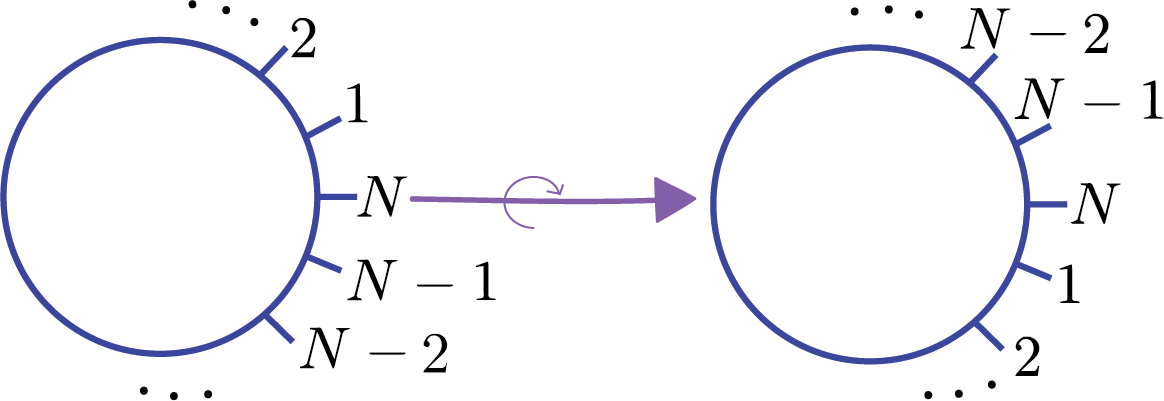
\includegraphics[width=0.6\textwidth]{Figures/Reflection_over_circle.png}
    \caption{Meaning of the relabel done in the circulant matrix, which can be seen as a reflection over the circle.}
    \label{reflectioncircle}
\end{figure}
Explicitly we can write that if $\tilde{\Gamma}^{+}_{mn}$ has the shape
\begin{equation}
\left(\begin{array}{ccccc}
a_{0} & a_{-1} & \cdots & a_{2} & a_{1} \\
a_{1} & a_{0} & \cdots & a_{3} & a_{2} \\
\cdot & \cdot & \cdot & \cdots & \cdot \\
\vdots & \vdots & \vdots & \vdots & \vdots \\
a_{-1} & a_{-2} & a_{-3} & \cdots & a_{0}
\end{array}\right),
\end{equation}
then $\tilde{\Gamma}^{-}_{mn}$ will be given by
\begin{equation}
\left(\begin{array}{ccccc}
a_{0} & a_{1} & \cdots & a_{-2} & a_{-1} \\
a_{1} & a_{2} & \cdots & a_{-1} & a_{0} \\
\cdot & \cdot & \cdot & \cdots & \cdot \\
\vdots & \vdots & \vdots & \vdots & \vdots \\
a_{-1} & a_{0} & a_{1} & \cdots & a_{-2}
\end{array}\right),
\end{equation}
which we name anticirculant.\\
\indent In this way, both the circulant and the anticirculant parts of $\Gamma$ are computed as Fourier transforms of the vectors $m^{+}(\theta_k)e^{i\phi(\theta_k)}$ and $m^{-}(\theta_k)e^{i\phi(\theta_k)}$ respectively.\\
\indent Here we spot 3 things. First, the FCM always can be written as a circulant matrix $\Gamma^{+}$ plus an anticirculant matrix $\Gamma^{-}$. Second, in the ground state, the FCM is circulant because the fermion occupation numbers $n^{c}\left(\theta_{k}\right)=n^{s}\left(\theta_{k}\right)=0, \forall k$. Third, for a generic excited state, we have that in average the FCM matrix is always circulant, because $\langle n^{c}\left(\theta_{k}\right)\rangle=\langle n^{s}\left(\theta_{k}\right)\rangle$.
\subsection{Local modes in the $XY$ model}
For our purpose, it is important to study the behaviour of reduced states in the chain, that is, we want to look into small portions of size $L$ in a translationally invariant chain of size $N$ ($N>L$). To do this it is convenient to write the modes of the small chain of size $L$ in terms of the modes of whole chain of size $N$.\\
 Since we work with a one-dimensional, translationally invariant closed chains of $N$ free fermions, with local interactions, it is often useful to expand the annihilation/creation operators $\hat{a}_x$ ($\hat{a}^{\dagger}_l$) at the site $x$ ($x = 0,1,\ldots, N-1$) in terms of their counterpart in the plane-wave basis, obtained through
\begin{equation}
\hat{b}_{q} = \frac{e^{i\eta_q}}{\sqrt{N}}\sum_{x=0}^{N-1}e^{-i\phi_q x}\hat{a}_x,
\end{equation}
and its hermitian conjugate, with $\phi_q = \frac{2\pi}{N}l$, and $\eta_q$ is a phase to be adjusted. By doing so, we showed that in the case of the $XY$ model, the Hamiltonian \eqref{CH2:Hamiltonian_jordan_wigner} became diagonal on the operators $\hat{b}_q$, explicitly we showed that the Hamiltonian had the form
\begin{equation}
\hat{H} = \sum_{q=0}^{N} \Lambda(\phi_q)\hat{b}_q^{\dagger}\hat{b}_q,
\label{CH2:Hamiltonian_diagonal}
\end{equation}
with $\Lambda(\phi_q)$ given by \eqref{CH3:Spectrum_XY_model} in the $XY$ model.\\
\indent We consider now a set of local plane wave modes for the portion of the chain of length $L$ comprising the sites $x=0,1,\ldots,L-1$,
\begin{equation}
\tilde{b}_k = (-1)^{k}\frac{e^{-i\tilde{\phi_k}/2}}{\sqrt{L}}\sum_{x=0}^{L-1}e^{-i\tilde{\phi}_k x}\hat{a}_x,
\end{equation}
where similarly as in the case of the large chain of size $N$, we take $\tilde{\phi}_k = \frac{2\pi}{L}k$. By introducing the modes of the local chain in this way, the plain wave modes will diagonalize any Hamiltonian of the form \eqref{CH2:Hamiltonian_diagonal}, with $N$ replaced by $L$.\\
\indent We now expand the local operators $\tilde{b}_k$ in terms of the global operators $\hat{b}_q$ that are defined over the chain of size $N$. The relation between the two becomes
\begin{equation}
\tilde{b}_k = \frac{1}{\sqrt{NL}}\sum_{q=0}^{N-1} D_{L}(\phi_q-\tilde{\phi}_k) \hat{b}_q,
\label{CH2:From_L_to_N}
\end{equation}
where we chose appropriately  $\eta_q = \phi_q(L-1)/2$, and
\begin{equation}
D_{L}(\phi) = \frac{\sin\left(\frac{\phi}{2}L\right) }{\sin\left(\frac{\phi}{2}\right)},
\end{equation}
is the Dirichlet kernel\cite{bashirov_chapter_2014}.\\
\indent Now consider an excited state $\ket{\vec{n}}$ of the chain, described by a set of excitation numbers $\vec{n}\equiv (n_0,n_1,\ldots, n_{N-1})$, where $n_q\in \{0,1\}$. In particular the state satisfies
\begin{equation}
\bra{\vec{n}}\hat{b}^{\dagger}_{q}\hat{b}_{q'}\ket{\vec{n}} = \delta_{q,q'}n_q,\quad \bra{\vec{n}}\hat{b}_{q}\hat{b}_{q'}\ket{\vec{n}} = \bra{\vec{n}}\hat{b}^{\dagger}_{q}\hat{b}^{\dagger}_{q'}\ket{\vec{n}} = 0,
\end{equation}
for all $q,q'$. To any excited state, we can associate the correspondent $L\times L$ FCM, that is
\begin{equation}
A_{kk'}(\vec{n}) = \bra{\vec{n}}\tilde{b}^{\dagger}_k \tilde{b}_{k'}\ket{\vec{n}} = \frac{1}{NL}\sum_{q=0}^{N-1}D_{L}(\phi_q-\tilde{\phi}_k)D_L(\phi_q-\tilde{\phi}_{k'})n_q.
\end{equation}
Therefore, we have a full characterization of any subchain in the state $\ket{\vec{n}}$, or equivalently in the state
\begin{equation}
\rho_L(\vec{n}) ) \operatorname{Tr}_{N-L} \ket{\vec{n}}\bra{\vec{n}},
\end{equation}
the corresponding partial density matrix on the subchain.
\section{Error correcting code theory}
\begin{figure}[H]
\centering
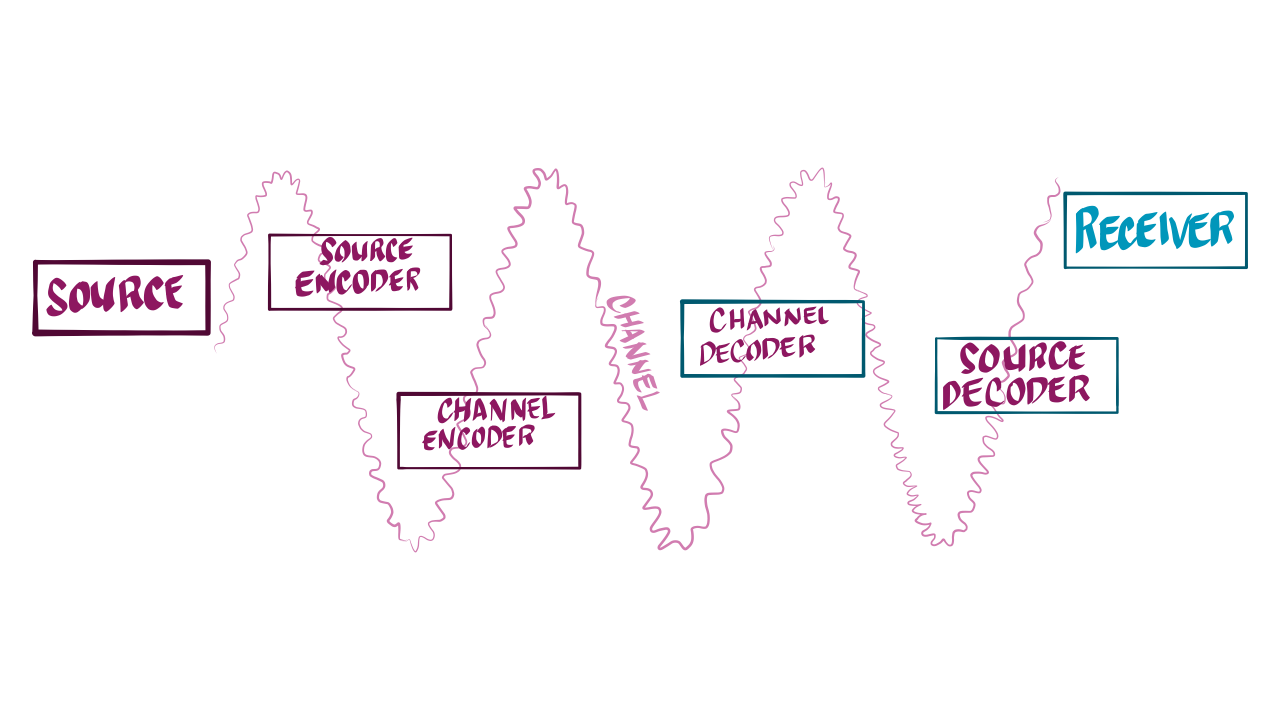
\includegraphics[width=0.7\textwidth]{Figures/Source_Destination.png}
\caption{Representation of the scheme of communication.The encoding system introduces some redundancy into the transmitted vector $\mathbf{x}$. The decoding system uses this known redundancy to deduce from the received vector $\mathbf{y}$ both the original source vector and the noise introduced by the channel.}
\label{CH2:Channel_communication}
\end{figure}
We will now turn to study error correcting codes. We start by motivating the problem of error correction codes as a mechanism to understand communication, then we move to introduce basic definitions to formalise the problem of error correcting codes. Afterwards, we will move to study the case of random minimum distance codes and some interesting results about them.\\
\indent Every day we communicate over noisy channels such as in cellphone lines, over which two devices communicate digital information. When we design these channels the main purpose is to be able to transmit information in a reliable way while dealing with  errors induced by the noise in the channel. Information theory and coding theory offer a way to study communications as C. Shannon pointed out in $1948$ \cite{shannon_mathematical_1948}. As we illustrate in figure \ref{CH2:Channel_communication}, we add encoders before the channel and decoders after it. The encoders encode the source message $\mathbf{x}$ into a transmitted message $\mathbf{y}$, adding redundancy to the original message in some way. The channel adds noise to the transmitted message, yielding a received message $\mathbf{y}$. The decoders use the known redundancy introduced by the encoding system to infer both the original signal $\mathbf{s}$ and the added noise.
\subsection{Channel coding}
\begin{figure}[H]
\centering
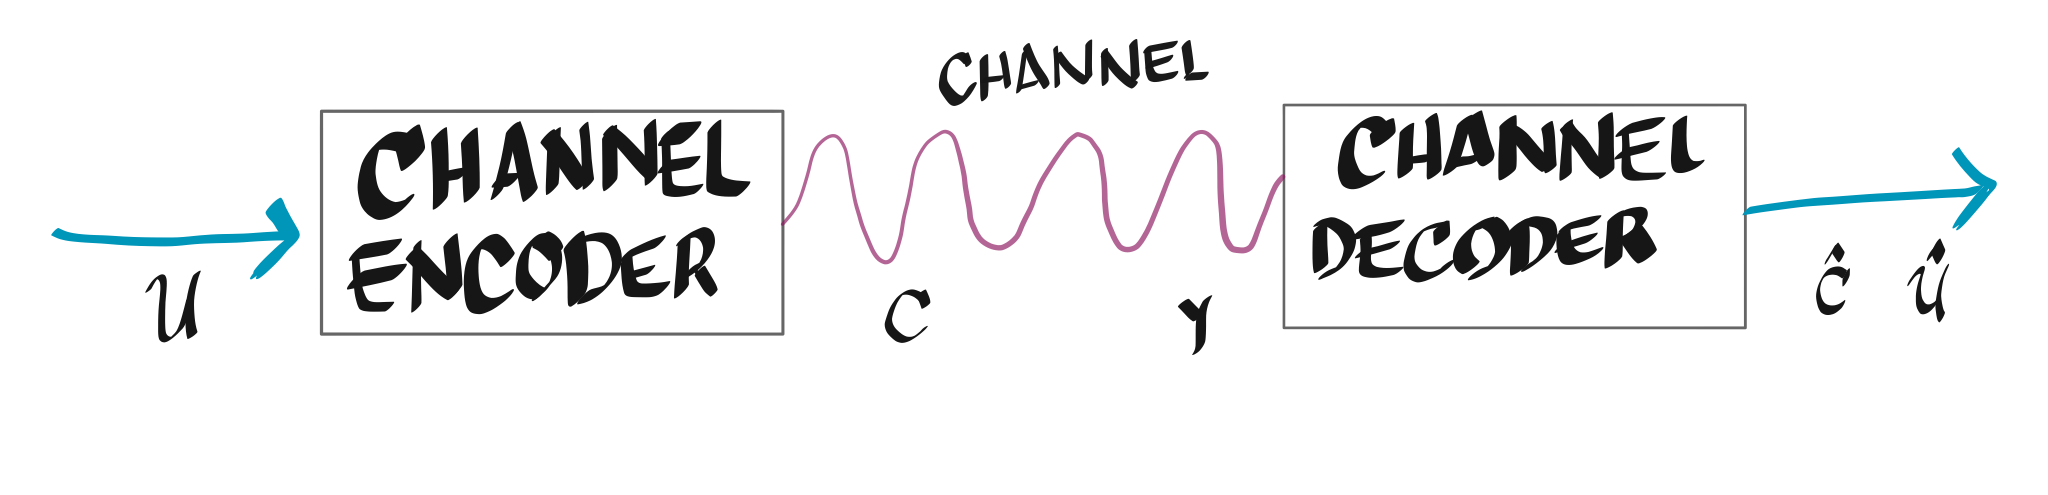
\includegraphics[width=0.8\textwidth]{Figures/Channel_decoder.png}
\caption{Channel coding}
\label{CH2:Channel_communication_2}
\end{figure}
For the purpose of our work, the model of channel we will use, is the \textit{discrete probability channel}: a probabilistic channel $S$ is defined as a triple $(F,\Phi,\operatorname{Prob})$, where $F$ is a finite \textit{input alphabet}, $\Phi$ is a finite \textit{output alphabet}, and $\operatorname{Prob}$ is a conditional probability distribution
\begin{equation}
\operatorname{Prob}\{\mathbf{x}|\mathbf{y}\},
\end{equation}
defined for every pair $(\mathbf{x},\mathbf{y})\in F^{m}\times\Phi^m$, where $m$ ranges over all positive integers and $F^m/\Phi^m$ denotes the set of all words of length $m$ over $F/\Phi$. It is important to clarify that we assume that the channel neither deletes nor inserts symbols; that is, the length of the output word $\mathbf{y}$ always equals the length of the input word $\mathbf{x}$.\\
\indent The input channel encoder is an \textit{information word} $\mathbf{u}$ out of $M$ possible information words (see figure \ref{CH2:Channel_communication_2}). The channel encoder generates a \textit{codeword} $\mathbf{c}\in F^n$ that is input to the channel. The resulting output of the channel is a received word $\mathbf{y}\in\Phi^n$, which is fed into the channel decoder. the decoder, in turn, produces a \textit{decoded codeword} $\hat{\mathbf{c}}$ and a \textit{decoded information word} $\hat{\mathbf{u}}$, with the aim of having $\mathbf{c}=\hat{\mathbf{c}}$ and $\mathbf{u}=\hat{\mathbf{u}}$. this implies that the channel encoder needs to be such that the mapping $\mathbf{u}\mapsto \mathbf{c}$ is one to one.
\begin{definition}[Rate]
The \textit{rate} of the channel encoder is defined as 
\begin{equation}
R = \frac{\log_{|F|}M}{n}.
\end{equation}
\end{definition}
If all information words have the same length over $F$, then this length is given by the numerator, $\log_{|F|}M$, in the expression for $R$. Since the mapping of the encoder is one-to-one, we have that $R\leq 1$.\\
In the case where the input alphabet $F$ has the same size as the output alphabet $\Phi$, it will be convenient to assume that $F=\Phi$ and that the elements of $F$ form a finite Abelian group. We then say that the channel is an \textit{additive channel}.\\
\indent Given an additive channel, let $\mathbf{x}$ and $\mathbf{y}$ be input and output words, respectively, both in $F^m$. the \textit{error word} is defined as the difference $\mathbf{x}-\mathbf{y}$, where the subtraction is taken component by component. The action of the channel can be described as adding an error word $\mathbf{e}\in F^m$ to the input word $\mathbf{x}$ to produce the output word $\mathbf{y} = \mathbf{x}+\mathbf{e}$, as shown in figure \ref{algo_2}.\\
\indent When $F$ is an Abelian group, it contains the zero (or unit) element. The \textit{error locations} are indexes of the nonzero entries in the error word $\mathbf{e}$. Those entries are referred to as the \textit{error values}.
\subsection{Block codes}
An $(n,M)$ (\textit{block}) code over a finite alphabet $F$ is a nonepty subset $\mathfrak{C}$ of size $M$ of $F^n$. The parameter $n$ is called the \textit{code length} and $M$ is the \textit{code size}. The \textit{information length} or \textit{codeword length} of $\mathfrak{C}$ is defined by $k=\log_{|F|}M$, and the \textit{rate} is $R=k/n$. the range of the mapping defined by the channel encoder in figure \ref{CH2:Channel_communication_2} forms an (n,M) code, and this in which the term $(n,M)$ code will be used. The elements of a code are called \textit{codewords}.\\
\indent In addition to the length and size of a code, we will be interested in quantifying how much the codewords in the code differ from each other. To do this, we will introduce the following definitions.
\begin{definition}[Hamming distance]
Let $F$ be an alphabet. The Hamming distance between two codewords $\mathbf{x},\mathbf{y}\in F^n$ is the number of coordinates on which $\mathbf{x}$ and $\mathbf{y}$ differ. the Hamming distance will be denoted by $d(\mathbf{x},\mathbf{y})$.
\end{definition}
\indent It is easy to verify that the Hamming distance satisfies the following properties of a metric for every three words $\mathbf{x},\mathbf{y},\mathbf{z}\in F^n$.
\begin{enumerate}[label=(\roman*)]
\item $d(\mathbf{x},\mathbf{y})=\geq 0$, with equality if and only if $\mathbf{x}=\mathbf{y})$.
\item Symmetry: $d(\mathbf{x},\mathbf{y})=d(\mathbf{y},\mathbf{x})$.
\item The triangle inequality: $d(\mathbf{x},\mathbf{y}) \leq d(\mathbf{x},\mathbf{z})+ d(\mathbf{z},\mathbf{y})$.
\end{enumerate}
\begin{definition}[Hamming weight]
Let $F$ be an Abelian group. The Hamming weight of $\mathbf{e}\in F^n$ is the number of nonzero entries in $\mathbf{e}$. We denote the Hamming weight by $w(\mathbf{e})$.
\end{definition}
\indent Notice that for every two words $\mathbf{x}, \mathbf{y}\in F^n$,
\begin{equation}
d(\mathbf{x},\mathbf{y}) = w(\mathbf{y}-\mathbf{x}).
\end{equation}
Turning back now to block codes, let $\mathfrak{C}$ be an $(n,M)$ code over $F$ with $M>1$. The \textit{minimum distance} of $\mathfrak{C}$ is the minimum Hamming distance between any two distinct codewords of $\mathfrak{C}$; that is, the minimum distance $d$ is given by
\begin{equation}
d=\min_{\mathbf{c}_1,\mathbf{c}_2\in \mathfrak{C} : \mathbf{c}_1\neq \mathbf{c}_2} d(\mathbf{c}_1,\mathbf{c}_2).
\end{equation}
An $(n,M)$ with minimum distance $d$ is often called $(n,M,d)$ code. We will sometimes use the notation $d(\mathfrak{C}))$ for the minimum distance of a given code $C$.\\



\subsection{Decoding}
Let $\mathfrak{C}$ be an $(n,M,d)$ code over an alphabet $F$ and let $S$ be the channel defined by the triple $(F,\Phi,\operatorname{Prob})$. A decoder for the code $\mathfrak{C}$with respect to the channel $S$ is a function
\begin{equation}
\mathcal{D}: \Phi^n\to \mathfrak{C}.
\end{equation}
The \textit{decoding error probability} $P_{\text{err}}$ of $\mathcal{D}$ is defined by
\begin{equation}
P_{\text{err}} = \max_{\mathbf{c}\in\mathfrak{C}} P_{\text{err}}(\mathbf{c}),
\end{equation}
where 
\begin{equation}
P_{\text{err}}(\mathbf{c}) = \sum_{\mathbf{y}:\mathcal{D}(\mathbf{y})\neq \mathbf{c}} \operatorname{Prob}\{\mathbf{y}\text{ received }|\mathbf{c}\text{ transmited}\}.
\end{equation}
Note that $P_{\text{err}}(\mathbf{c}$ is the probability that the code word $\mathbf{c}$ will be decoded erroneously, given that $\mathbf{c}$ was transmitted
\subsubsection{Maximum-likelihood decoding}

\indent Information theory is concerned with the theoretical limitations of reliable communication, meaning that is always asking. ``What is the best error-correcting performance we could achieve?''\\
\indent Coding theory is concerned with the creation of practical encoding and decoding systems.




 Thus, encoding is the process of adding redundancy and decoding is the process of removing errors and the communication can only be done over the channel\cite{mackay_information_2003}. The most fundamental question one can ask is what will be the relation between the amount of redundancy and the errors that can be corrected, and in order to answer this question we will provide some useful definitions.

\indent The relative distance of $C$, denoted $\delta(C)$, is the quantity $\frac{\Delta(C)}{N}$, where $N$ is the block length of $C$. Thus, any two code words of $C$ differ in at least a fraction $\delta(C)$.
\begin{definition}[Notation]
 A q-ary code of block length $N$ and dimension $k$ will be referred to as an $[N,k]_q$ code. Further, if the code has minimum distance $d$, it will be referred to as an $[N,k,d]_q$ code. When the alphabet size $q$ is clear from the context, or not very relevant to the discussion, we omit the subscript.
\end{definition}

\indent Up to this point we have only described specific definitions for codes, codes with fixed block length and dimension. However, since we are interested in the asymptotic behaviour, it turns out to be more useful to study families of codes instead of an specific code.

\begin{definition}[Family of Codes]
 Let $q\geq 2$. let $\{n_i\}_{i\geq 1}$ be and increasing sequence of block lengths and suppose there exists sequences $\{k_i\}_{i\geq 1}$ and $\{d_i\}_{i\geq 1}$ such that for all $i\geq 1$ there exist an $[n_i,k_i,d_i]_q$ code $C_i$. then the sequence $C=\{C_i\}_{i\geq1}$ is a family of codes. The asymptotic rate of C is defined as
\begin{equation}
R(C)=\lim _{i \rightarrow \infty}\left\{\frac{k_{i}}{n_{i}}\right\},
\label{CH2:Rate_of_family_code}
\end{equation}
and the asymptotic relative distance of $C$ is defined as
\begin{equation}
\delta(C)=\lim _{i \rightarrow \infty}\left\{\frac{d_{i}}{n_{i}}\right\},
\label{CH2:Relative_distance_of_family_code}
\end{equation}
from now on whenever we talk about a code we will implicitly refer to an associated family of codes.
\end{definition}
\indent Our purposes of this work, we are going to focus on a particular class of codes, namely minimum distance codes. This special kind of codes came to our interest because they seem to appear naturally when study typical Fermionic states. We will then show some of the main results on this particular kind of codes to after show how this results could be extended to our particular case.\\

\indent Codes of minimum distance $d$ are codes that have the property that for every pair $x,y$ of codewords we have that
\begin{equation}
\Delta(x,y) \geq d,
\end{equation}
and therefore, all relative distances $\delta$ satisfy by $n\delta=d$.\\

\indent When working with this kind of codes one may wonder what is the best rate we can achieve. Particularly we are going to show three results, one positive and two negative results\footnote{Note that a negative result refer to an upper bound on the rate, meaning that the maximum achievable rate we could get can not exceed some value. Whereas a positive result refer to  lower bound on the rates we can achieve.}. Even though there are other known bounds, we will not talk about others but Gilbert-Varshamov, Hamming and Plotkin bounds, the reason for this is due to the fact that the other bound apply for large enough alphabets, so for binary codes we are not interested at all in these kind of bounds\cite{mackay_information_2003}.
\begin{figure}
\centering
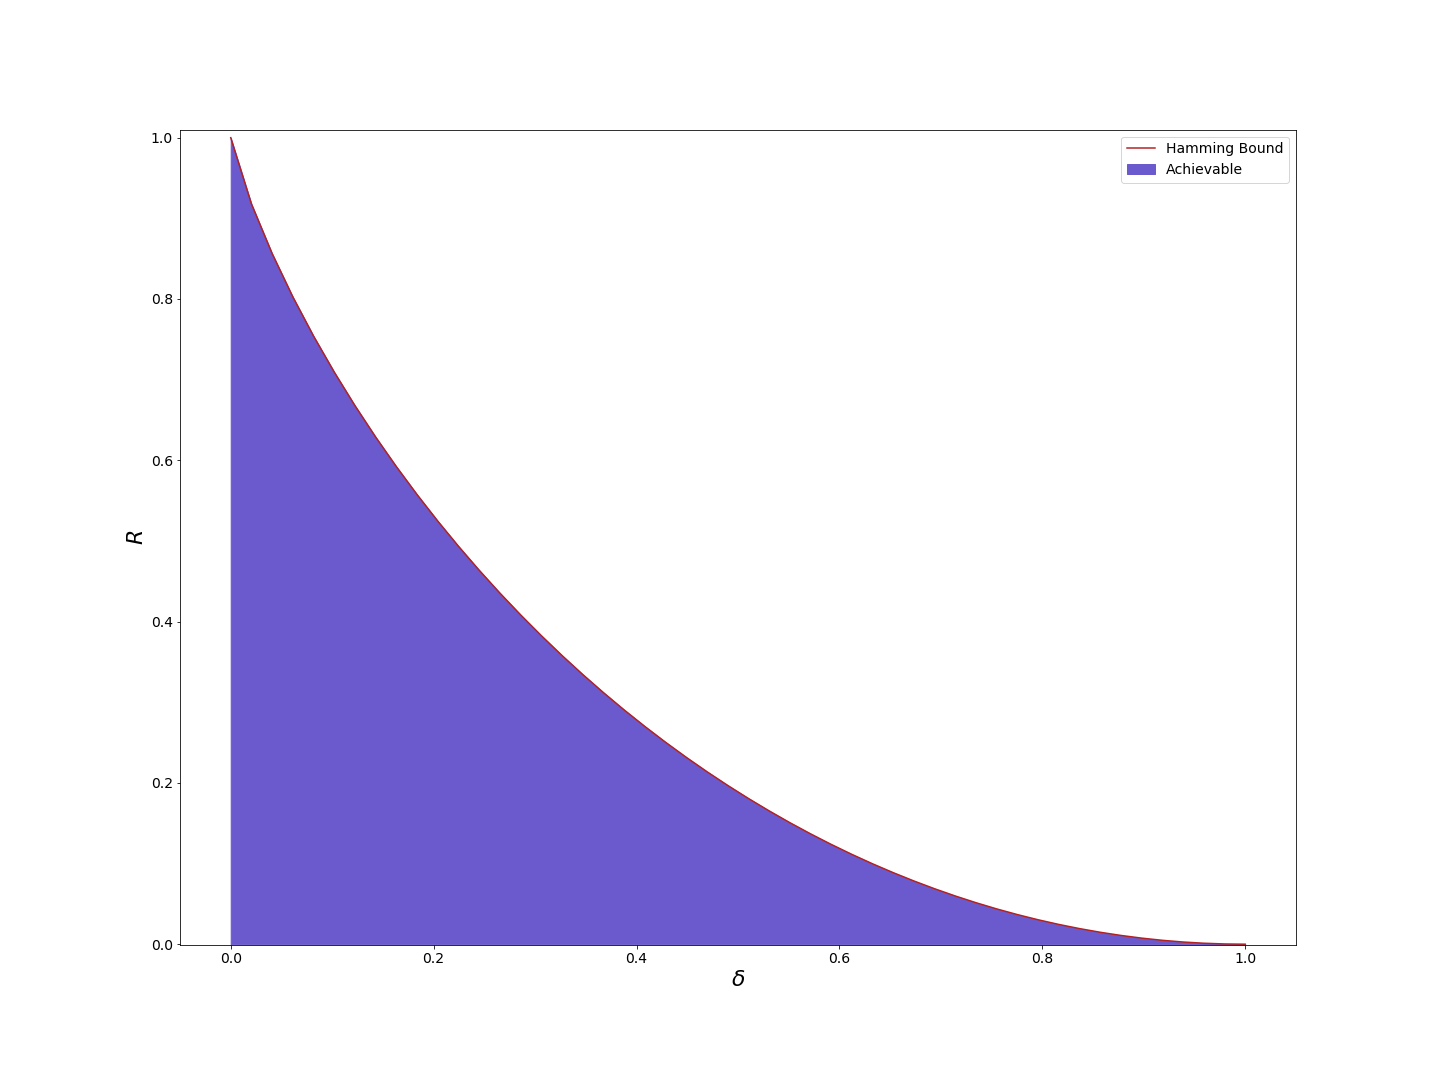
\includegraphics[width=0.7\textwidth]{Figures/Hamming_bound.png}
\caption{An illustration of the Hamming bound for the case of $q=2$. Note any code above this bound could exist. The shaded region shows the codes that could exist.  }
\end{figure}
\subsection{Hamming Bound (Sphere packing bound)}
\begin{definition}[Volume of Hamming ball]
\indent Let $ q\geq2$ and $n \geq r \geq 1$ be integers. Then the volume of a Hamming ball of radius $r$ is given by
\begin{equation}
\operatorname{Vol}_{q}(r, n)=\left|B_{q}(\mathbf{0}, r)\right|=\sum_{i=0}^{r}\left(\begin{array}{l}
n \\
i
\end{array}\right)(q-1)^{i},
\label{CH2:Hamming_ball}
\end{equation}
where the choice of $\mathbf{0}$ as the center of the Hamming ball is chosen arbitrary, since the volume of the Hamming ball is independent of its center.
\end{definition}
\indent It is simple to show that
\begin{equation}
\frac{k}{n} \leq 1-\frac{\log _{q} \operatorname{Vol}_{q}\left(\left\lfloor\frac{d-1}{2}\right\rfloor, n\right)}{n},
\label{CH2:Hamming_bound_1}
\end{equation}
where the volume in \eqref{CH2:Hamming_bound_1} correspond to the definition in\eqref{CH2:Hamming_ball}. With some algebra and using the Stirling asymptotic approximation one can show that
\begin{equation}
\operatorname{Vol}_{q}\left(\left\lfloor\frac{d-1}{2}\right\rfloor, n\right) \geq q^{H_{q}\left(\frac{\delta}{2}\right) n-o(n)},
\end{equation}
where the latter inequality immediately provide us an upper bound on the rate
\begin{equation}
R \leq 1-H_{q}\left(\frac{\delta}{2}\right)+o(1).
\label{CH2:Hamming_bound_2}
\end{equation}

\indent The inequality in \eqref{CH2:Hamming_bound_2} is known as the Hamming Bound.

\subsection{Plotkin Bound}
\begin{definition}[Plotkin Bound]
The following holds for any code $\mathcal{C}\subset [q]^n$ 
\begin{itemize}
\item If $d=\left(1-\frac{1}{q}\right) n,|\mathcal{C}| \leq 2 q n$.
\item If $d>\left(1-\frac{1}{q}\right) n,|\mathcal{C}| \leq \frac{q d}{q d-(q-1) n}$.
\end{itemize}
Note that the Plotkin Bound implies that a code with relative distance $\delta\geq 1-1/q$, must necessarily have $R=0$.
\end{definition}

\begin{definition}
For any q-ary code with relative distance $0 \leq \delta \leq 1-\frac{1}{q}$,
\begin{equation}
R \leq 1-\left(\frac{q}{q-1}\right) \delta+o(1).
\label{CH2:Plotkin_bound}
\end{equation}
\end{definition}

\begin{figure}
\centering
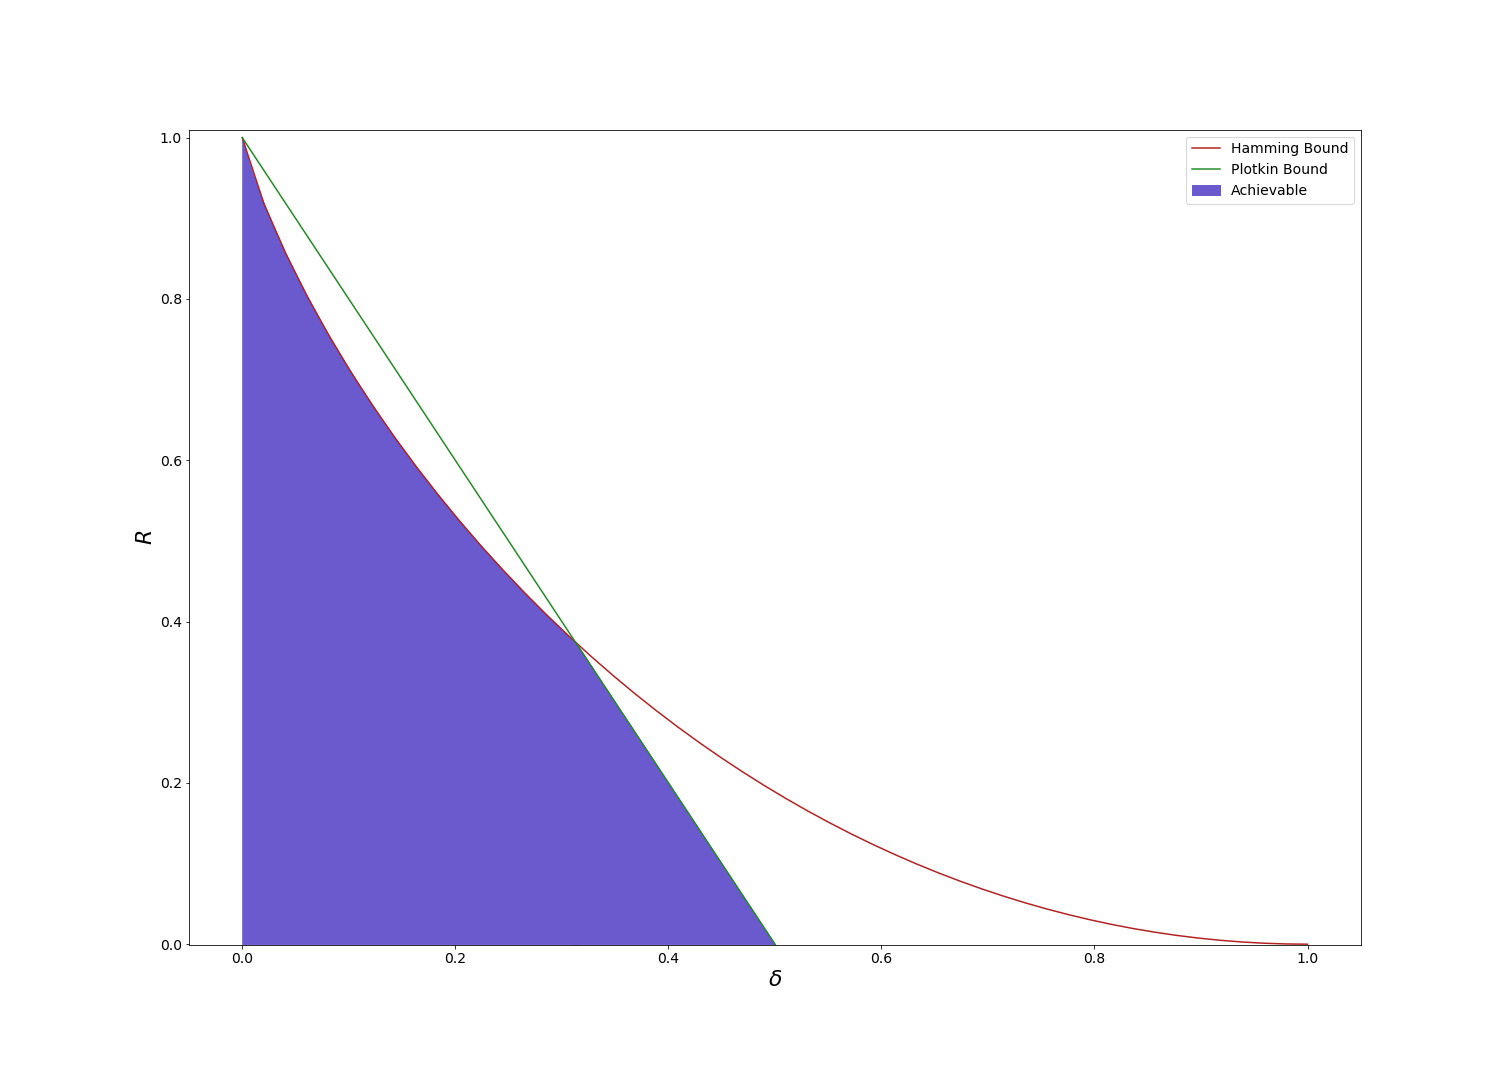
\includegraphics[width=0.7\textwidth]{Figures/Hamming_plotkin_bound.png}
\caption{An illustration of Plotkin and Hamming bounds for the case of $q=2$.  For this case the shaded region changes indicating us that there are not codes with $R>0$ when $\delta=1-1/q$ .}
\end{figure}

\indent To illustrate the proof of this bound we can consider the distance $d=n\delta$. So we can shorten the codewords and group them in a way such that they agree on the first $n-n'$ symbols, with $n^{\prime}=\left\lfloor\frac{q d}{q-1}\right\rfloor-1$. Then in particular for any $x\in [q]^{n-n'}$, define the prefix code
\begin{equation}
\mathcal{C}_{\mathbf{x}}=\left\{\left(c_{n-n^{\prime}+1}, \ldots c_{n}\right) \mid\left(c_{1} \ldots c_{N}\right) \in \mathcal{C},\left(c_{1} \ldots c_{n-n^{\prime}}\right)=\mathbf{x}\right\}.
\end{equation}
for all $x,\ \mathcal{C}_{x}$, has distance $d$ as $\mathcal{C}$ has distance $d$. Additionally, it has block length $n^{\prime}<\left(\frac{q}{q-1}\right) d$, and thus $d>\left(1-\frac{1}{q}\right) n^{\prime}$. From the Plotkin bound, this implies that
\begin{equation}
\left|\mathcal{C}_{\mathbf{x}}\right| \leq \frac{q d}{q d-(q-1) n^{\prime}} \leq q d,
\end{equation}
where the second inequality follows from the fact that $q d-(q-1) n^{\prime}$ is an integer.\\

\indent Note that the definition of $\mathcal{C}_{x}$
\begin{equation}
|\mathcal{C}|=\sum_{\mathbf{x} \in[q]^{n-n^{\prime}}}\left|\mathcal{C}_{\mathbf{x}}\right|,
\end{equation}
tells us that 

\begin{equation}
\left.|\mathcal{C}| \leq \sum_{\mathbf{x} \in[q]^{n-n^{\prime}}} q d=q^{n-n^{\prime}} \cdot q d \leq q^{n-\frac{q}{q-1} d+o(n)}=q^{n\left(1-\delta \cdot \frac{q}{q-1}+o(1)\right)}\right.,
\end{equation}

so, this provides another upper bound to the rate given by
\begin{equation}
R \leq 1-\left(\frac{q}{q-1}\right) \delta+o(1)
\label{CH2:Plotkin:bound_rate}
\end{equation}
\indent To close this section we will show the latter but positive result which provide us  lower bound on the code rates, Gilbert Varshamov bound.
\subsection{Gilbert-Varshamov Bound}
We now switch gears to provide a positive result. We will only provide the main ideas for the proof of this result an we will discuss why this result turn out to be one of the most important results.
\begin{definition}[Gilbert-Varshamov Bound]
Let $q\geq 2$. For every $0 \leq \delta<1-\frac{1}{q}$ and $0<\varepsilon \leq 1-H_{q}(\delta)$. There exists a code with rate $R \geq 1-H_{q}(\delta)-\varepsilon$ and relative distance $\delta$.
\label{CH2:Definition_Gilbert_Varshamov}
\end{definition}

\begin{figure}
\centering
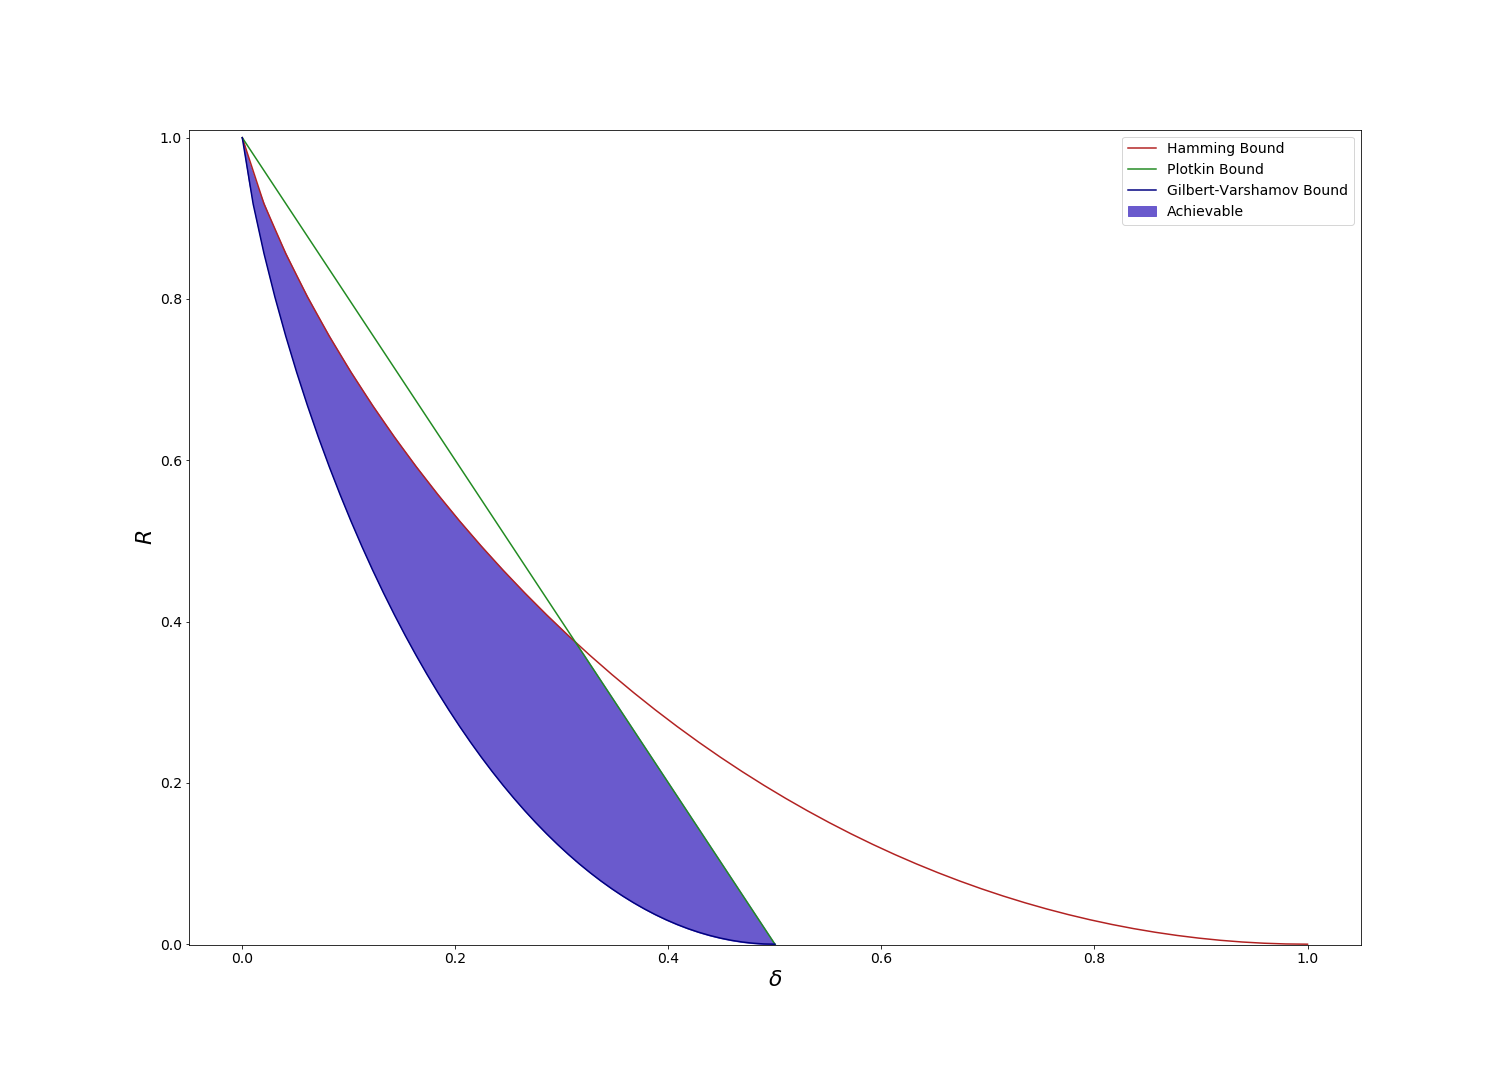
\includegraphics[width=0.7\textwidth]{Figures/Hamming_plotkin_Gilbert_bound.png}
\caption{An illustration of 3 bounds Hamming, Plotkin and Gilbert-Varshamov for the case of $q=2$. The lower bound correspond to the Gilvert-Varshamov Bound whereas the other 2 are the upper bound for the rate.}
\end{figure}

\indent To provide a sketch of about the proof we can consider a greedy approach. First we start with an empty code $\mathcal{C}$ and we keep adding vectors that are not in $\mathcal{C}$ and that have Hamming distance at least $d$ from all the existing codewords in $\mathcal{C}$. Notice that by doing so we can assure that we will never add a vector $c$ that will make that will make the distance of $\mathcal{C}$ fall below $d$. Indeed it is easy to see that after doing so, we have
\begin{equation}
\bigcup_{\mathbf{c} \in C} B(\mathbf{c}, d-1)=[q]^{n};
\label{CH2:Gilbert_Varshamov_1}
\end{equation}
This is easily checked, since if it were not true, then there would exist a vector $\mathbf{v} \in[q]^{n} \backslash C$, such that $\Delta(\mathbf{v}, \mathbf{c}) \geq d$ and therefore $\mathbf{v}$ could be added. However, this would contradict the fact that we have finished the procedure. So

\begin{equation}
\bigcup_{c \in C} B(\mathbf{c}, d-1) \mid=q^{n}.
\label{CH2:Gilbert_Varshamov_2}
\end{equation}
Also, It isn't hard to see that
\begin{equation}
\sum_{\mathbf{c} \in C}|B(\mathbf{c}, d-1)| \geq\left|\bigcup_{\mathbf{c} \in C} B(\mathbf{c}, d-1)\right|,
\label{CH2:Gilbert_Varshamov_3}
\end{equation}
which implies that
\begin{equation}
\sum_{\mathbf{c} \in C}|B(\mathbf{c}, d-1)| \geq q^{n},
\label{CH2:Gilbert_Varshamov_4}
\end{equation}
but as mentioned before, the volume of the Hamming ball is translation invariant,

\begin{equation}
\sum_{\mathbf{c} \in C} \operatorname{Vol}_{q}(d-1, n) \geq q^{n}.
\label{CH2:Gilbert_Varshamov_5}
\end{equation}
Since $\sum_{\mathbf{c} \in C} V o l_{q}(d-1, n)=V o l_{q}(d-1, n) \cdot|C|$ 

\begin{equation}
\begin{aligned}
|C| & \geq \frac{q^{n}}{\operatorname{Vol}_{q}(d-1, n)} \\
& \geq \frac{q^{n}}{q^{n H_{q}(\delta)}} \\
&=q^{n\left(1-H_{q}(\delta)\right)}.
\end{aligned}
\label{CH2:Gilbert_Varshamov_final}
\end{equation}

Therefore concluding the proof. It is worth mentioning that this way of proceeding the code does not any special structure, but as one might think, this algorithm will take exponentially long time to finish. However, one may wonder if there is a special kind of code that also achieves this rate. Indeed is possible to show that \textit{random linear codes} lies, with high probability, on the Gilbert-Varshamov Bound. To pick a \textit{random linear code} we only need pick a random $k\times n $ matrix, in which each entry is chosen uniformly and independently at random according to its alphabet\cite{mackay_information_2003,jaynes_probability_2003}. Aside from these result providing some bounds on the rate of the minimum distance codes. We are interested in the performance of a special kind of random codes, more specifically binary codes over a binary-symmetric channel (BSC). Here, we derive the minimum distance, distance distribution and error exponent of a typical random code (TRC) from a random code ensemble (RCE), as well as the one correspondent to a typical linear code (TLC) from a linear code ensemble (LCE) \cite{barg_random_2002}. As mentioned by A Barg, and G. D. Forney, Jr \cite{barg_random_2002} most of the important results are expressed in terms of the Gilbert-Varshamov distance  $\delta_{GV}(R)$.
\subsection{Error Exponents for Random Minimum Distance Codes}
It is very well known that on a BSC with crossover probability $p$, the channel capacity is $C=1-H_2(p)$ \footnote{We will be using the notation $\mathcal{H}$ to refer to the binary entropy $\mathcal{H}\equiv H_2$ }. The coding error exponent $E_r(R)$ is positive for $0\leq R < C$ and given by \cite{gallager_low-density_1962,gallager_information_1968}.
\begin{equation}
E_{r}(R)=\left\{\begin{array}{ll}
R_{0}-R, & 0 \leq R \leq R_{\text {crit }} \\
E_{\mathrm{sp}}(R), & R_{\text {crit }} \leq R \leq C
\end{array}\right.,
\end{equation}
where $R_0$,  $R_{\text {crit }}$ and $E_{\mathrm{sp}}(R)$, are known as the cutoff rate, the critical rate and the sphere-packing exponent, respectively. Gallager has shown \cite{gallager_random_2006},that the random coding exponent is the true error exponent for the RCE   on any discrete memoryless channel. Here we will show the main results provided in \cite{barg_random_2002} and we will provide the ideas to derive these results, as we will show later this ideas of error exponents will be quite helpful to understand how it is possible to make a connection between minimum distance codes and typical Fermionic  states.
\subsubsection{Random Binary Codes}
Consider a binary code $C$ of length $n$ and rate $R$ bits per symbol is a set of $M=2^{NR}$. For the case of RCE one computes the probability that by taking a random codeword $\mathbf{x}_i$ of length $N$ it would have Hamming distance $d=N\delta$ from an arbitrary binary $N-$tuple $\mathbf{b}$ and see that it will be independent of $\mathbf{b}$ and equals to
\begin{equation}
\text{Pr}\{d_H(\mathbf{x}_i,\mathbf{b})=d\}={N\choose d} \tilde{p}^d (1-\tilde{p})^{N-d},
\end{equation}
where $\tilde{p}$ corresponds to the probability of having a one. Under this RCE, two distances $d_H(\mathbf{x}_i,\mathbf{x}_j)$ and $d_H(\mathbf{x}_{i'},\mathbf{x}_{j'})$ are independent random variables. So if we consider the number of unordered pairs of codewords $(\mathbf{x}_i,\mathbf{x}_j)$ with $i\neq j$ in $C$ at a distance $d$ apart
\begin{equation}
S_{\mathcal{C}}(d)=\sum_{i=0}^{M-1} \sum_{j=0}^{i-1} \Phi\left\{d_{H}\left(\boldsymbol{x}_{i}, \boldsymbol{x}_{j}\right)=d\right\},
\end{equation}
where $\Phi\left\{d_{H}\left(\boldsymbol{x}_{i}, \boldsymbol{x}_{j}\right)=d\right\}$ is equal to 1 if the condition $d_H(\mathbf{x}_i,\mathbf{x}_j)$ is satisfied and $0$ otherwise. For the case of RCE on a BSC $S_{\mathcal{C}}(d)$ is a sum of ${M\choose 2}$ pairwise independent, identically distributed random variables, so we have

\begin{equation}
\mathrm{E} S_{\mathcal{C}}(d)=\left(\begin{array}{c}
M \\
2
\end{array}\right) \mathrm{E} \Phi \doteq 2^{N(2 R-1+\mathcal{H}(\delta))}.
\end{equation}
\indent Therefore we are ready to state the following theorem
\begin{theorem}[Minimum distance in RCE]
For $0\leq R< 1/2$ and any $\varepsilon>0$, the probability that a code length $N$ and rate $R$ from the RCE has relative minimum distance less than $\delta_{GV}(2R)-\varepsilon$ goes to zero exponentially as $N\to \infty$. For $0\leq R < 1$, if $d=N\delta$ is such that
\begin{equation}
\delta_{GV}(2R)+\varepsilon \leq \delta \leq 1- \delta{GV}(2R) - \varepsilon,
\end{equation}
then the probability that the number of codeword pairs at a distance d satisfies $S_{\mathcal{C}}(d) \doteq 2^{N(2 R-1+\mathcal{H}(\delta))}$ goes to one as $N\to \infty$.
\end{theorem}

\begin{proof}
For a given value of the code value of the code rate $R$ we can choose $d$ such that $d/N\to\delta \leq \delta_{\mathrm{GV}}(2 R)-\varepsilon$. Then
\begin{equation}
\operatorname{Pr}\left\{S_{\mathcal{C}}(d) \geq 1\right\} \leq \mathrm{E} S_{\mathcal{C}}(d) \doteq 2^{-N(1-\mathcal{H}(\delta)-2 R)} \rightarrow 0,
\end{equation}
which in other words tells us that with probability differing from $1$ by an exponentially falling quantity, there will be no pairs at distance $d$. Notwithstanding this result, if $\delta_{\mathrm{GV}}(2 R)+\varepsilon<\delta<1-\delta_{\mathrm{GV}}(2 R)-\varepsilon$, then $1-\mathcal{H}(\delta)<2R$ and the average of number of pairs $\mathrm{E} S_{\mathcal{C}}(d)$ at a distance $d$ is exponentially large. To see this, we can use the Chebyshev inequality, so for any $\delta>0$, we have 
\begin{equation}
\operatorname{Pr}\left\{\left|S_{\mathcal{C}}(d)-\mathrm{E} S_{\mathcal{C}}(d)\right| \geq\left(\begin{array}{c}
M \\
2
\end{array}\right) \alpha\right\} \leq \frac{\mathrm{E} \Phi}{\left(\begin{array}{c}
M \\
2
\end{array}\right) \alpha^{2}};
\end{equation}
by choosing $\alpha \doteq 2^{-N(1-\mathcal{H}(\delta)+\Delta)}<\mathrm{E} \Phi$ for any $\Delta>0$, we have
\begin{equation}
\operatorname{Pr}\left\{\left|S_{\mathcal{C}}(d)-\mathrm{E} S_{\mathcal{C}}(d)\right|>\left(\begin{array}{c}
M \\
2
\end{array}\right) \alpha\right\}\leq \frac{2 \mathrm{E} \Phi}{M(M-1) \alpha^{2}} \doteq 2^{-N(2 R-1+\mathcal{H}(\delta)-2 \Delta)}.
\end{equation}
The exponent on the right-hand side can be made positive by choosing $\Delta$ small enough. This establishes the fact that $S_{\mathcal{C}}(d)\doteq 2^{N(2 R-1+\mathcal{H}(\delta))}$ for the chosen value of $d$ with probability tending to one as $N\to\infty$.
\end{proof}
\subsubsection{Random Linear Codes}
A binary linear code $C$ of length $n$ and rate $K/n$ is a set of $M=2^K$ binary $n$-tuples that is generated by $K$ $n-$linerarly independent tuples $\mathbf{g}_j$, $1\leq k \leq K$. This is
\begin{equation}
\mathbf{x}(u)=\Sigma_k \mathbf{u}_k \mathbf{g}_j,
\end{equation}
where $\mathbf{u}$ is an arbitrary binary $K-$tuple. Here we will be considering the case in which each of the $2^{NK}$ matrices are chosen with equal probability. For the case of linear codes, the distance distribution $\{d_H(\mathbf{x}_i,\mathbf{x}_j),i\neq j\}$ from any given codeword $\mathbf{x}_i$ is independent of $i$. The average distance distribution of a linear code $C$ therefore reduces to
\begin{equation}
\mathcal{N}_{\mathcal{C}}(d)=\sum_{j \neq i} \Phi\left\{d_{H}\left(\boldsymbol{x}_{i}, \boldsymbol{x}_{j}\right)=d\right\} \quad(d=1,2, \ldots, N),
\label{CH2:RLC_number of codewords}
\end{equation}
where $\mathbf{x}_i$ is an arbitrary codeword. Typically, $\mathbf{x}_i$ is taken as the all zero codeword $\mathbf{0}=\mathbf{x(0)}$. If $(\mathbf{u}_j,\mathbf{u}_k)$ is any pair distinct non-zero $K-$tuples, then the corresponding codewords $(\mathbf{x}(\mathbf{u}_j),\mathbf{x}(\mathbf{u}_k))$ are a pair of independent random binary $N-$tuples. It follows that two distinct distances $d_H(\mathbf{x}_i,\mathbf{x}_j)$ and $d_H(\mathbf{x}_i,\mathbf{x}_k)$ from a given codeword $\mathbf{x}_i$ are pairwise-independent and distributed as in the RCE. In particular 
\begin{equation}
\operatorname{Pr}\left\{d_{H}\left(\boldsymbol{x}_{i}, \boldsymbol{x}_{j}\right)=N \delta\right\} \doteq 2^{-N(1-\mathcal{H}(\delta))},
\end{equation}
for any $d=N\delta$, the quantity $\mathcal{N}_{\mathcal{C}}(d)$ in \eqref{CH2:RLC_number of codewords} is a sum of $M-1\doteq 2^{NR}$ pairwise-independent, identically distributed random variables with mean $E\Phi\doteq 2^{-N(1-mathcal{H}(\delta))}$. Its mean value is therefore equal to

\begin{equation}
\mathcal{N}_{\mathrm{LCE}}(d) \doteq 2^{N(R-1+\mathcal{H}(\delta))}.
\end{equation}
Therefore we say that the relative minimum distance of a code chosen at random from the LCE will be, with probability $1-2^{-\Omega(N)}$, approximately equal to the $GV$ relative distance $\delta_{GV}(R)$.\\

\indent In summary, the typical minimum distance in the LCE is better than that in the RCE because the minimum of only $M-1$ pairwise-independent distances, whereas in the RCE it is the minimum of ${M\choose 2}$ pairwise independent distances.\\

\indent Up to this point one may be wonder how all this theory of correcting errors and minimum distance codes are connected to our problem. In following section we are going to show how this connection emerges as a natural consequence of the structure in the Clifford algebra and therefore provide an explanation of what we named as ultra orthogonality.







\indent We have presented details about some generalities in quadratic Hamiltonians, the equivalence between $1/2-$spin systems and fermions, and how fermionic systems described by \eqref{CH2:QuadraticHamiltonian} can be brought to its diagonal form, to be analytically solved. In the next chapter we will expound some historical background concerning  error correcting code theory, as well as some of the most relevant results in the bounds in minimum distance codes. Once we have explained all the tools of code theory that will be needed, we will show how is possible to connect the formalism we discussed in this chapter with code theory, and interpret Fermionic states as binary sequences of excitations, to prove that is possible to find exponentially large Hilbert spaces in which ultra-orthogonality will holds. 


